\chapter{Obsah CD}
\label{pr:cd}
Adresárová štruktúra CD
\begin{itemize}
\item \textit{src} - Zdrojové súbory
    \begin{itemize}
    \item \textit{web} - Webový portál
    \item \textit{api} - Javascriptové API
    \item \textit{game} - Hra
    \item \textit{test} - Testovací skript
    \item \textit{database} - Databázový skript
    \item \textit{demo} - Demo aplikácia s už prichystanými nastaveniami, obsahujúca hru, jej materiály a funkčné API. (pre ľahšiu inštaláciu a demonštráciu)
    \end{itemize}
\item \textit{text} - Text práce
\end{itemize}

\chapter{Návod na inštaláciu}
\label{instalacia}
Keďže aplikácia využíva rámec Nette a ten má isté požiadavky, tak server, na ktorom sa bude aplikácia nachádzať musí tieto požiadavky splňovať. Tieto požiadavky je možné overiť Requirements-Checker skriptom, viac informácií na stránke s oficiálnou dokumentáciou\footnote{https://doc.nette.org/cs/2.3/requirements}. Ďalej je nutné mať v internetovom prehliadači povolený Javascript pre správny chod platformy a vôbec pre spustenie HTML5 hier. Demonštračná hra vyžaduje taktiež splnené určité požiadavky, v prvom rade je to existencia canvas tagu, znova viac informácií v repozitáry rámca\footnote{https://github.com/photonstorm/phaser\#requirements}.
\section{Inštalácia}
\begin{enumerate}
\item V prvom rade je nutné v phpMyAdmin, alebo inom, spustiť skript databa.sql, ktorý sa nachádza na priloženom CD v priečinku database. Tento skript vytvorí potrebné tabuľky a naplní ich dátami ukážkovými dátami. 
\item Ďalej je nutné nahrať obsah priečinku demo (obsahuje demo aplikáciu už s hrou, pre ľahkú demonštráciu) na server a upraviť súbor v app/config/config.local.neon s prístupovými údajmi k databáze. 
\item Pre správne fungovanie Aplikačného rámca je nutné ďalej nastaviť adresu, na ktorú sa bude API dotazovať. Ak je napríklad domovská stránka webu načítaná po zadaní adresy www.example.com, tak práve túto adresu treba nastaviť do API súboru, riadok 8/9 premenná server v súbore api/api.js. Okrem toho, je to potrebné nastaviť ešte v totožnom súbore nachádzajúci sa v upload/games/1/js/api.js pre správne fungovanie demonštračnej hry.
\end{enumerate}

\chapter{Dokumentácia k API}
\label{pr:dokumentacia}
\section{Funkcie}
\begin{itemize}
\item \textbf{initialize(key[, callback[, context]]) –} funkcia slúžiaca na inicializáciu API na strane servera. 
\begin{itemize}
\item \textbf{Parametre funkcie:} API kľúč získaný z vývojárskej konzole z detailu hry, callback, ktorý je vykonaný po získaní odpovede, referencia na objekt, ktorý chceme v callbacku využívať. 
\item \textbf{Vracia:} data['status'] je 0 v prípade úspechu, 1 v prípade, že doména nie je povolená a 2 v prípade že hra neexistuje.
\end{itemize}

\item \textbf{login(username, password[, callback[, context]]) –} funkcia slúžiaca na prihlásenie hráča.
\begin{itemize}
\item \textbf{Parametre funkcie:} meno a heslo prihlasovaného hráča, callback, ktorý je vykonaný po získaní odpovede, referencia na objekt, ktorý chceme v callbacku využívať. 
\item \textbf{Vracia:} data['status'] je 0 v prípade úspechu, 1 v prípade, že je zadané nesprávne meno, alebo heslo a 2 v prípade, že užívateľ je už prihlásený. data['result'] vracia v prípade úspechu prezývku hráča.
\end{itemize}

\item \textbf{logout([callback[, context]]) –} funkcia slúžiaca na odhlásenie hráča.
\begin{itemize}
\item \textbf{Parametre funkcie:} callback, ktorý je vykonaný po získaní odpovede, referencia na objekt, ktorý chceme v callbacku využívať. 
\item \textbf{Vracia:} data['status'] je 0 v prípade úspechu, 1 v prípade, že užívateľ nie je prihlásený.
\end{itemize}

\item \textbf{isLogged([callback[, context]]) –} funkcia na zistenie, či je hráč prihlásený.
\begin{itemize}
\item \textbf{Parametre funkcie:} callback, ktorý je vykonaný po získaní odpovede, referencia na objekt, ktorý chceme v callbacku využívať. 
\item \textbf{Vracia:} data['status'] je 0 v prípade, že užívateľ je prihlásený, 1 v prípade, že užívateľ nie je prihlásený. data['result'] v prípade že je užívateľ prihlásený obsahuje jeho prezývku.
\end{itemize}

\item \textbf{postScore(table, value) –} funkcia na vloženie hodnoty skóre do tabuľky.
\begin{itemize}
\item \textbf{Parametre funkcie:} id tabuľky, do ktorej chceme vkladať skóre a hodnota skóre. 
\item \textbf{Vracia:} data['status'] je 0 v prípade úspechu, 1 v prípade, že tabuľka neexistuje, 98 v prípade, že užívateľ nieje prihlásený.
\end{itemize}

\item \textbf{getUserBestScore(table[, callback[, context]]) –} funkcia na získanie najvyššieho skóre daného prihláseného hráča.
\begin{itemize}
\item \textbf{Parametre funkcie:} id tabuľky, z ktorej chceme skóre získať, callback, ktorý je vykonaný po získaní odpovede, referencia na objekt, ktorý chceme v callbacku využívať. 
\item \textbf{Vracia:} data['status'] je 0 v prípade úspechu, 1 v prípade, že tabuľka neexistuje, 98 v prípade, že užívateľ nieje prihlásený. data['result'] v prípade úspechu obsahuje najvyššiu skóre hodnotu užívateľa z danej tabuľky.
\end{itemize}

\item \textbf{getScores(table, count[, callback[, context]]) –} funkcia na získanie prvých X miest zo skóre tabuľky.
\begin{itemize}
\item \textbf{Parametre funkcie:} id tabuľky, z ktorej chceme skóre získať, počet hodnôt, ktoré chceme získať, callback, ktorý je vykonaný po získaní odpovede, referencia na objekt, ktorý chceme v callbacku využívať. 
\item \textbf{Vracia:} data['status'] je 0 v prípade úspechu, 1 v prípade,m že tabuľka neexistuje. data['result'] v prípade úspechu obsahuje pole s užívateľmi a ich skóre.
\end{itemize}

\item \textbf{getAchievements([callback[, context]]) –} funkcia na získanie odmien a informácie o tom, či dané odmeny vlastní, alebo nevlastní aktuálne prihlásený hráč.
\begin{itemize}
\item \textbf{Parametre funkcie:} callback, ktorý je vykonaný po získaní odpovede, referencia na objekt, ktorý chceme v callbacku využívať. 
\item \textbf{Vracia:} data['result'] obsahuje odmeny.
\end{itemize}

\item \textbf{unlockAchievement(achievement[, callback[, context]]) –} funkcia na získanie/odblokovanie odmeny.
\begin{itemize}
\item \textbf{Parametre funkcie:} id odmeny, ktorú chceme, získať callback, ktorý je vykonaný po získaní odpovede, referencia na objekt, ktorý chceme v callbacku využívať. 
\item \textbf{Vracia:} data['status'] je 0 v prípade úspechu, 1 v prípade, že odmena neexistuje, 2 v prípade, že užívateľ už odmenu vlastní, 98 v prípade, že užívateľ nieje prihlásený. data['result'] v prípade úspechu obsahuje danú získanú odmenu.
\end{itemize}

\item \textbf{store(storage, value) –} funkcia na uloženie hodnoty do definovaného úložiska.
dané odmeny vlastní, alebo nevlastní aktuálne prihlásený hráč.
\begin{itemize}
\item \textbf{Parametre funkcie:} id úložiska, do ktorého chceme ukladať hodnotu a samotná hodnota 
\item \textbf{Vracia:} data['status'] je 0 v prípade úspechu, 1 v prípade, že úložisko neexistuje, 98 v prípade, že užívateľ nieje prihlásený.
\end{itemize}

\item \textbf{load(storage[, callback[, context]]) –} funkcia na získanie odmeny z definovaného úložiska.
\begin{itemize}
\item \textbf{Parametre funkcie:} id úložiska, callback, ktorý je vykonaný po získaní odpovede, referencia na objekt, ktorý chceme v callbacku využívať. 
\item \textbf{Vracia:} data['status'] je 0 v prípade úspechu, 1 v prípade, že úložisko neexistuje, 2 v prípade, že hodnota v úložisku neexistuje, 98 v prípade, že užívateľ nieje prihlásený. data['result'] v prípade úspechu obsahuje užívateľovu hodnotu z úložiska.
\end{itemize}

\section{Príklady}
\end{itemize}
\begin{lstlisting}[]
//Load value from storage
this.game.api.load(1, function(data, room){
    if(data['status'] == 2) //value does not exist
    {
        //Store to storage
        room.game.api.store(1, 1);
    }
    else //value exist
    {
        //Store to storage
        room.game.api.store(1, parseInt(data['result']) + 1);
    }
}, this);
\end{lstlisting}

\begin{lstlisting}[]
//Get user best score from score table
room.game.api.getUserBestScore(1, function(data, room) {
    room.game.playerBestScore = data['result']; //value from server
    room.hudBestScore = room.game.add.text(room.game.width*(3/4) + 100, room.game.height, "Best Score: " + data['result'], { font: '20px Arial', fontWeight: 'bold', fill: "#000000", align: "center" });
    room.hudBestScore.anchor.setTo(0.5,1);
}, room);
\end{lstlisting}

\begin{lstlisting}[]
//Unlock achievement
this.game.api.unlockAchievement(2, function(data, game) {
    if(data['status'] == 0) //achievement unlocked with success
    {
        achievement = game.add.text(game.width/2, game.height/2 - 100, data['result']['name'] + "\n Unlocked", { fontWeight: 'bold',font: '30px Arial', fill: "#000000", align: "center" });
        achievement.anchor.setTo(0.5);
        var fade = game.add.tween(achievement);
        fade.to( { alpha: 0 }, 4000, "Linear", true);
    }
}, this.game);
\end{lstlisting}

\chapter{Ukážky z implementácie}
\label{pr:implementacia}
\begin{figure}[h]
  \centering
  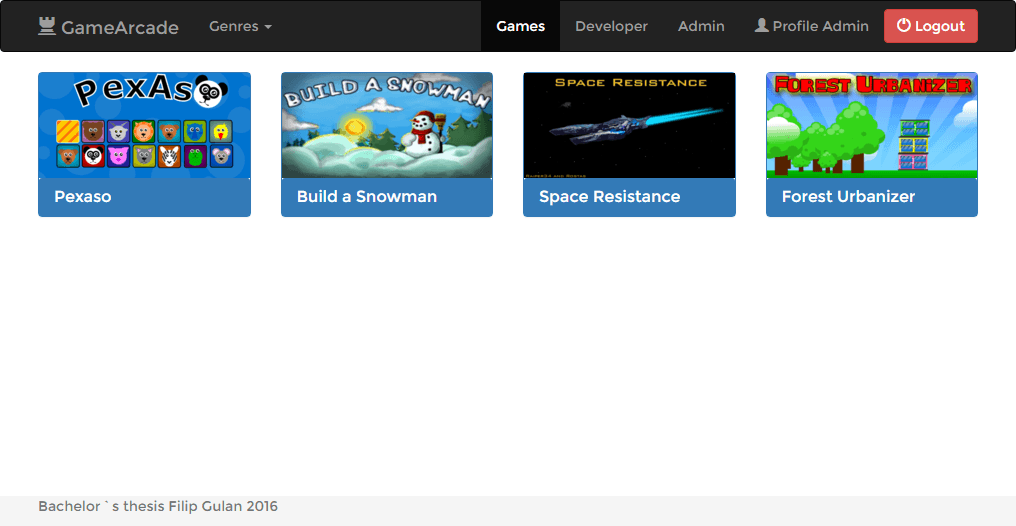
\includegraphics[scale=0.35]{fig/ukazka-zoznam-hier.png}
  \caption{Ukážka obrazovky so zoznamom hier. Hore na lište vedľa textového loga sa nachádza filtrovanie podľa žánru.}
  \label{fig:ukazka-zoznamhier}
\end{figure}

\begin{figure}[h]
  \centering
  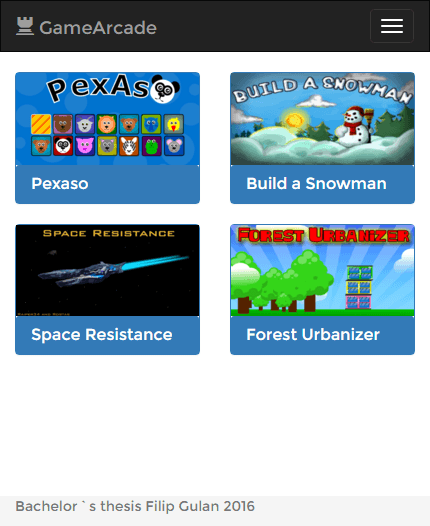
\includegraphics[scale=0.35]{fig/ukazka-responzivity.png}
  \caption{Ukážka zoznamu hier a jeho responzívnosti.}
  \label{fig:ukazka-zoznamhierresponzivny}
\end{figure}

\begin{figure}[h]
  \centering
  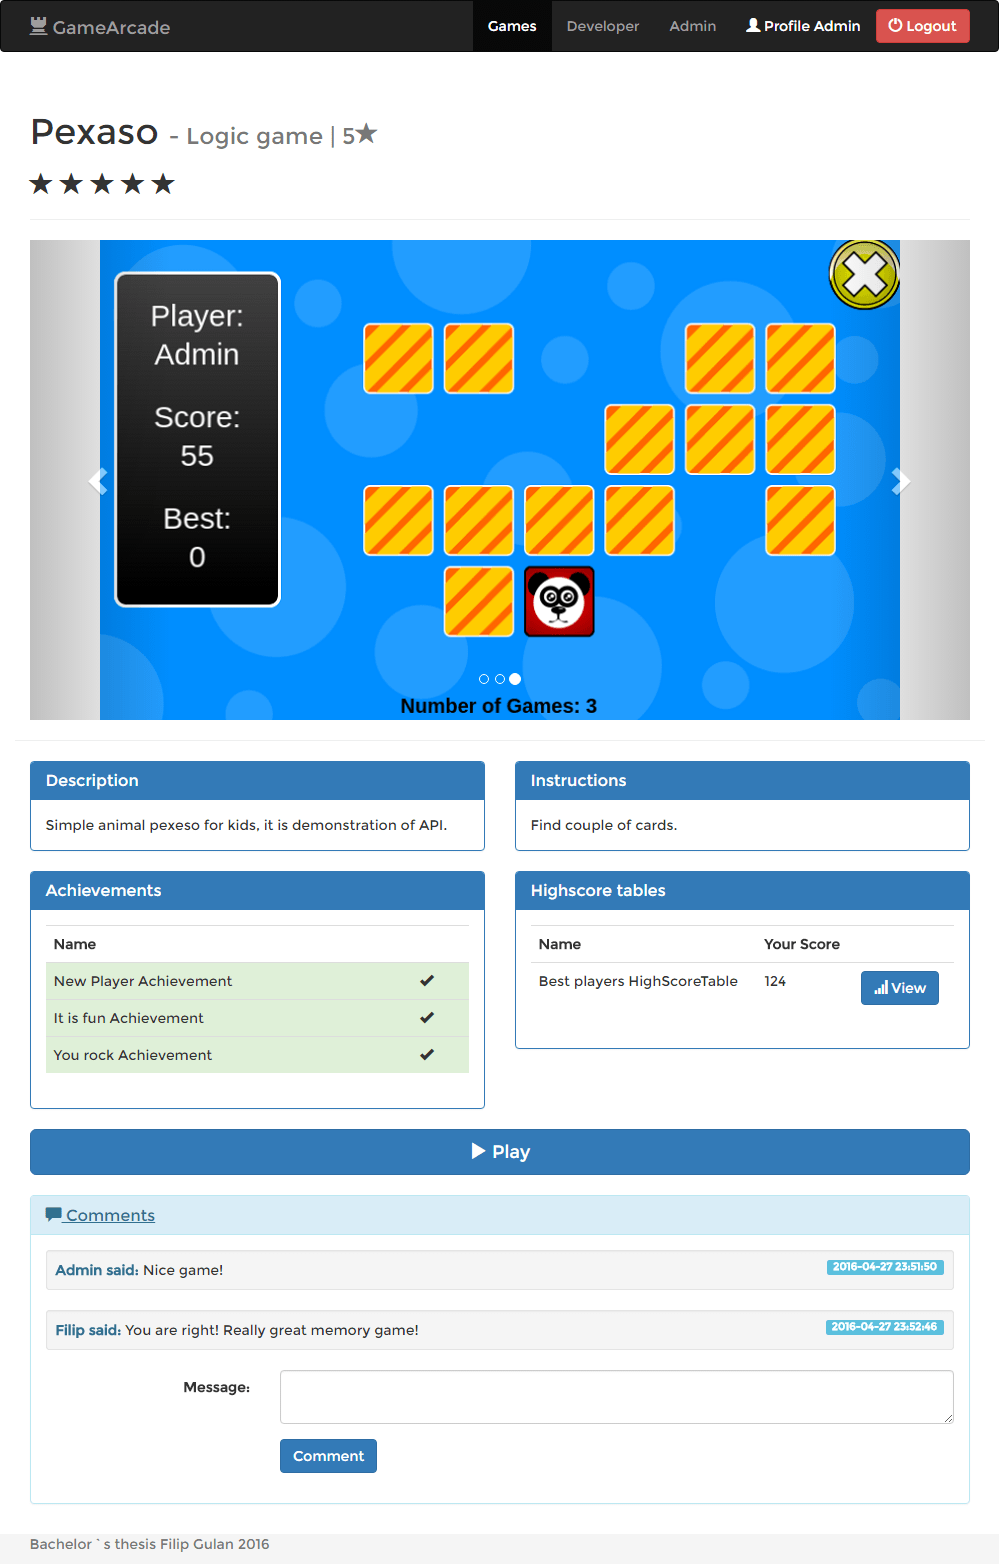
\includegraphics[scale=0.35]{fig/ukazka-detail-hra.png}
  \caption{Ukážka detailu hry. Nachádzajú sa tu panely s s jednotlivými informáciami (napríklad panel s odmenami, tabuľkami...)}
  \label{fig:ukazka-detailhry}
\end{figure}

\begin{figure}[h]
  \centering
  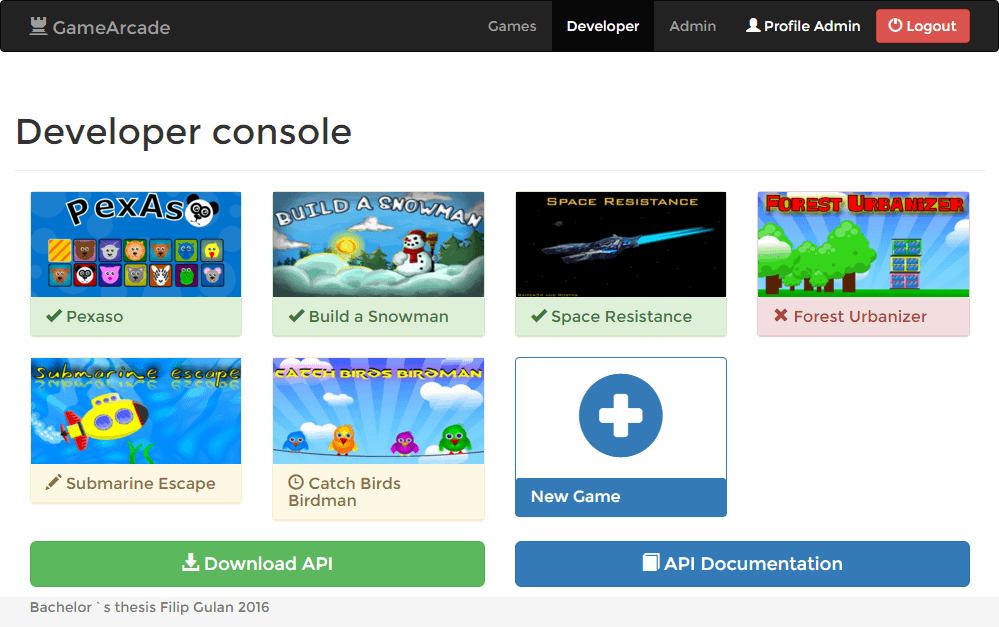
\includegraphics[scale=0.35]{fig/ukazka-zoznam-vyvojar.png}
  \caption{Ukážka vývojárskej konzole. Je možné vidieť hry v rôznom štádiu publikácie, ktorých panely sú farebne odlíšené.}
  \label{fig:ukazka-vyvojar}
\end{figure}

\begin{figure}[h]
  \centering
  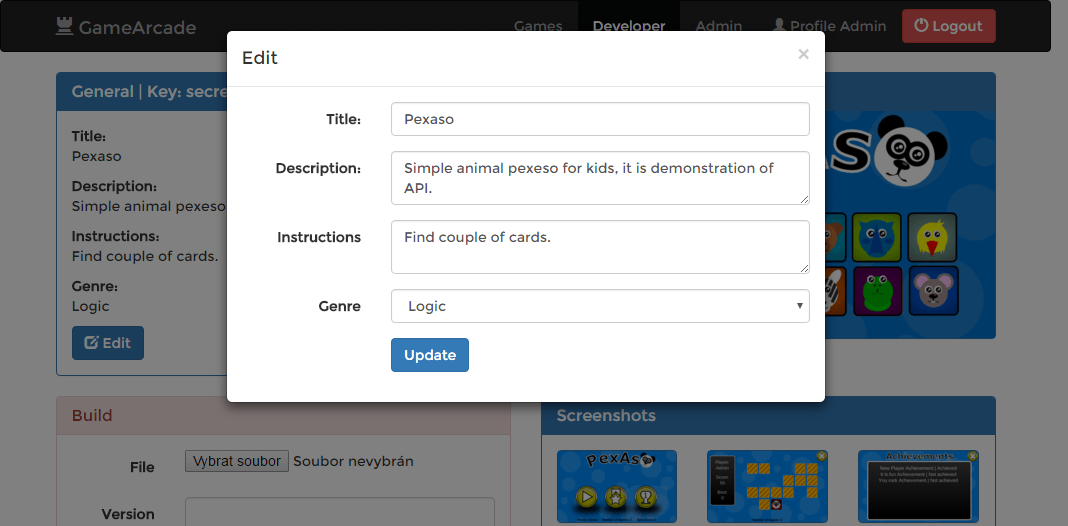
\includegraphics[scale=0.35]{fig/ukazka-modalne-okno.png}
  \caption{Ukážka úpravy informácií v detailu hry vo vývojárskej konzoly pomocou modálneho okna.}
  \label{fig:ukazka-modalneokno}
\end{figure}

\begin{figure}[h]
  \centering
  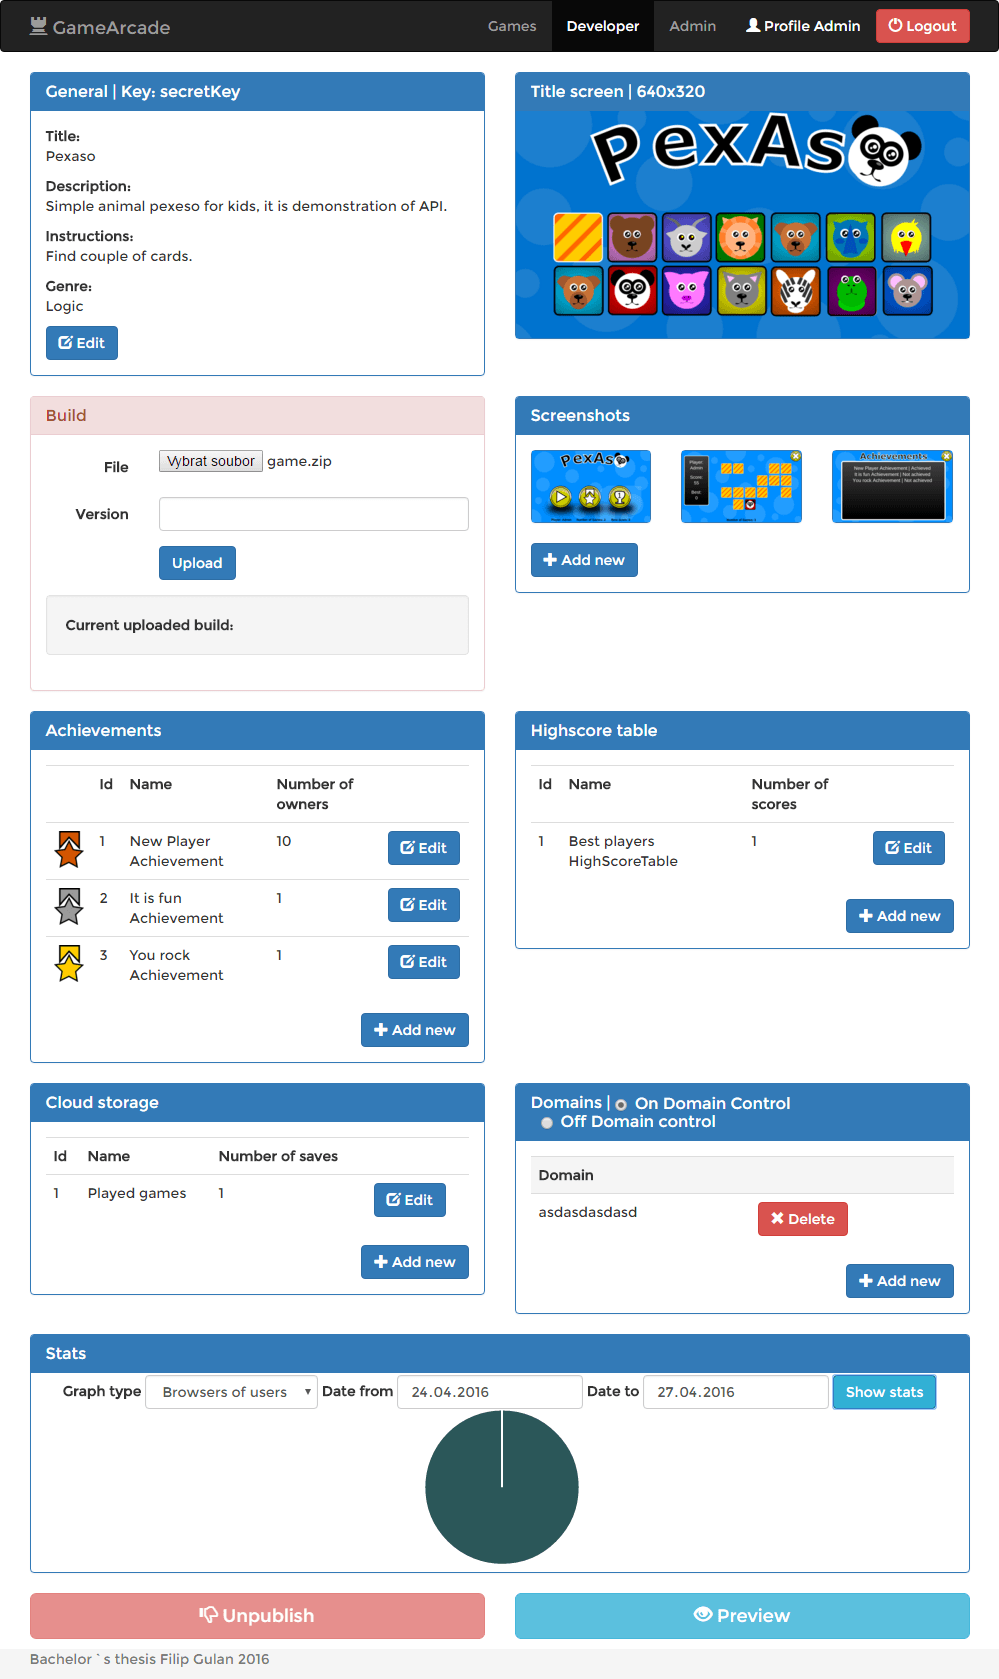
\includegraphics[scale=0.35]{fig/ukazka-detail-vyvojar.png}
  \caption{Ukážka detailu hry vo vývojárskej konzoly. Je možné vidieť jednotlivé panely, ktoré logicky oddeľujú jednotlivé informačné a editačné sekcie.}
  \label{fig:ukazka-detialvyvojar}
\end{figure}

\begin{figure}[h]
  \centering
  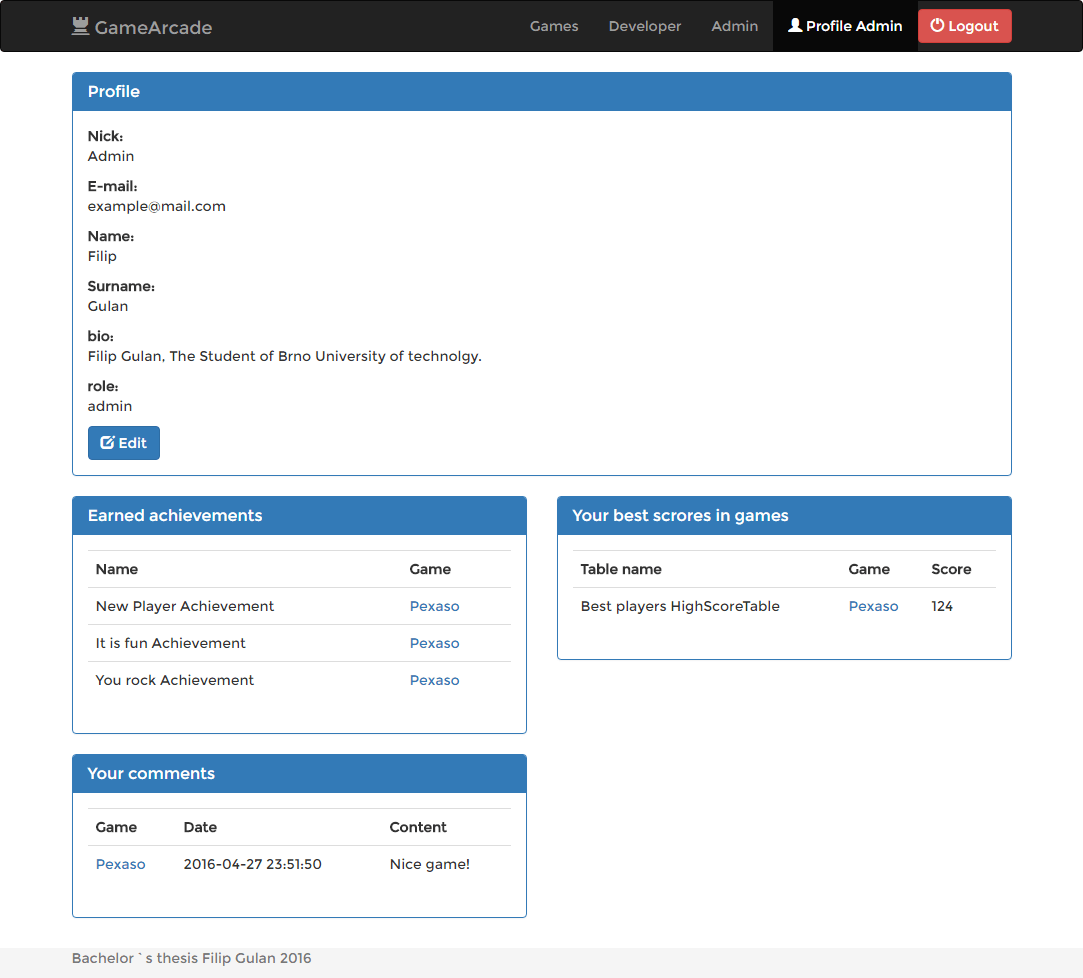
\includegraphics[scale=0.33]{fig/ukazka-profil.png}
  \caption{Ukážka profilu užívateľa.}
  \label{fig:ukazka-profil}
\end{figure}

\begin{figure}[h]
  \centering
  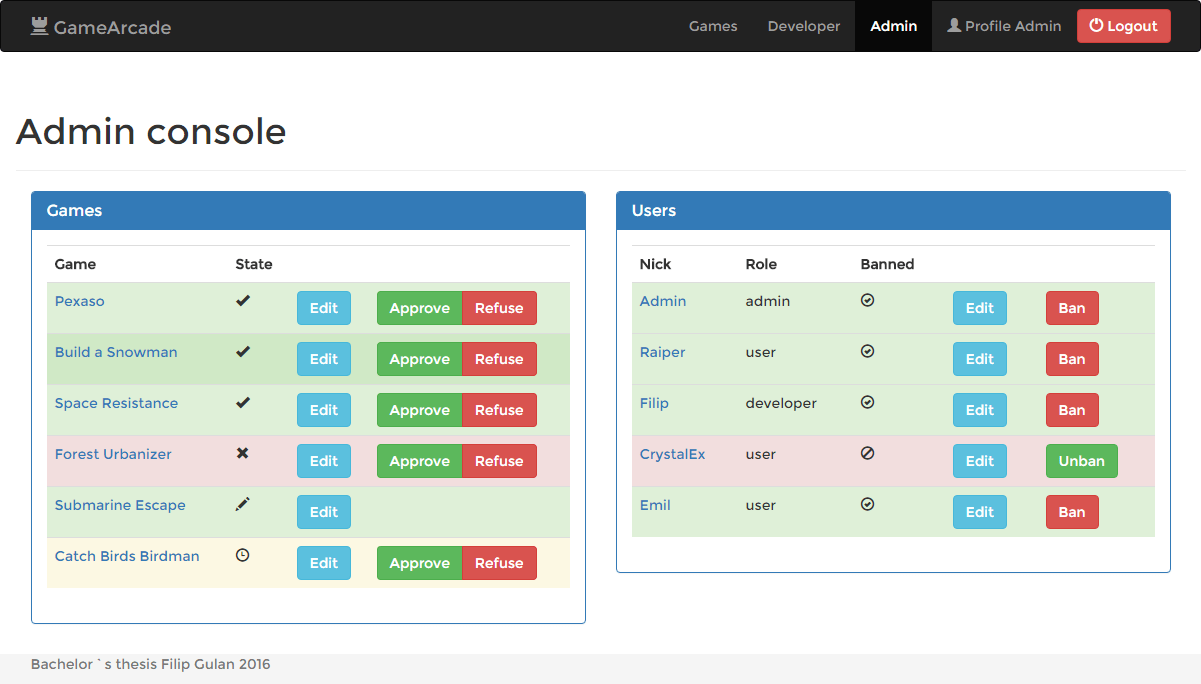
\includegraphics[scale=0.35]{fig/ukazka-admin.png}
  \caption{Ukážka administrátorskej konzoly. Je možné vidieť farebne odlíšené hry v jednotlivých štádiách publikácie a užívateľov, taktiež farebne odlíšených, podľa toho, či sú povolený, alebo zakázaný.}
  \label{fig:ukazka-admin}
\end{figure}

\begin{figure}[h]
  \centering
  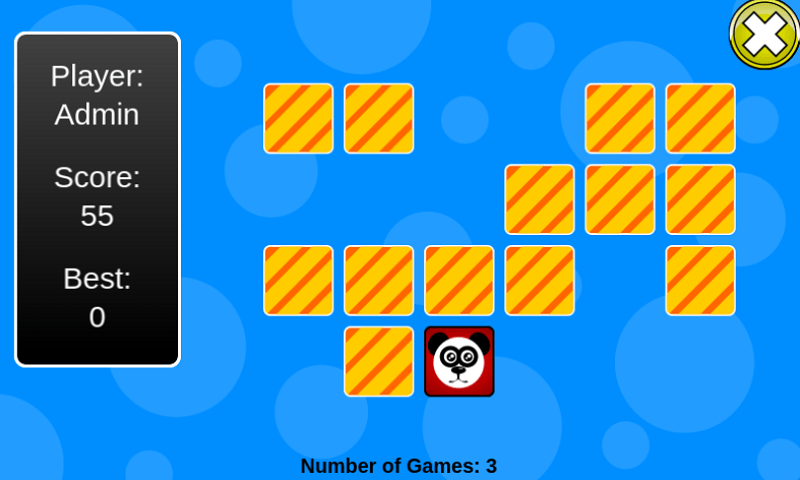
\includegraphics[scale=0.45]{fig/ukazka-hra.png}
  \caption{Ukážka levelu v demonštračnej hre. Naľavo je možné vidieť informačný panel, s informáciami, ktoré sú získané zo serveru pomocou implementovaného API.}
  \label{fig:ukazka-hra}
\end{figure}

\begin{figure}[h]
  \centering
  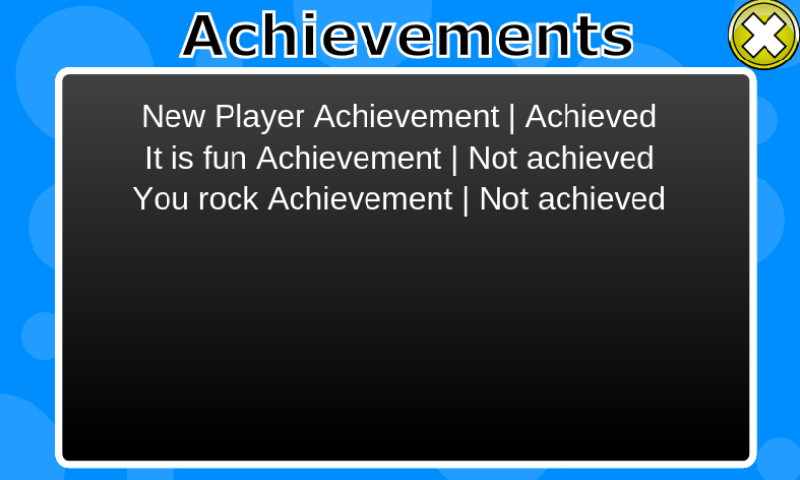
\includegraphics[scale=0.45]{fig/ukazka-hra-odmeny.png}
  \caption{Ukážka hernej obrazovky s odmenami. Obsahuje meno domény a informáciu o tom, či ju aktuálne prihlásený užívateľ získal.}
  \label{fig:ukazka-hraodmen}
\end{figure}




